%%%%%%%%%%%%%%%%%%%%%%%%%%%%%%%%%%%%%%%%%%%%%%%%%%%%%%%%%%%%%%%%%%%%%%%%%%%%%%%
% Chapter 2: Desarrollo
%%%%%%%%%%%%%%%%%%%%%%%%%%%%%%%%%%%%%%%%%%%%%%%%%%%%%%%%%%%%%%%%%%%%%%%%%%%%%%%

%++++++++++++++++++++++++++++++++++++++++++++++++++++++++++++++++++++++++++++++

En el cap\'{\i}tulo anterior se ha definido el Trabajo de Fin de Grado, especificado los objetivos y actividades
a desarrollar y mencionado las tecnolog\'{\i}as empleadas para su desarrollo. A continuaci\'on, se describir\'a 
la metodolog\'{\i}a de trabajo seguida y se introducir\'a a los resultados obtenidos para posteriormente
describirlos por cap\'{\i}tulos de manera detallada.

%++++++++++++++++++++++++++++++++++++++++++++++++++++++++++++++++++++++++++++++

\section{Metodolog\'{\i}a usada}
\label{2:sec:1}

Se ha llevado a cabo una metodolog\'{\i}a de trabajo \textit{\'agil}, com\'un en el campo de la \ceit{Ingenier\'{\i}a Inform\'atica},
con reuniones semanales en las que se defin\'{\i}an una serie de tareas u objetivos (iteraci\'on) y que se presentaban la siguiente semana. 
De este modo, con la entrega de prototipos funcionales de la \ceit{aplicaci\'on}, se han ido testeando, corrigiendo y mejorando las 
funcionalidades, al mismo tiempo que detectando problemas no contemplados en las fases previas de dise�o.

Esta metodolog\'{\i}a, adem\'as, ha propiciado la generaci\'on de ideas que se han traducido en nuevas caracter\'{\i}sticas.

%---------------------------------------------------------------------------------
\subsection{GitHub}
\label{subsec:2.1.1}

Para llevar a cabo esta metodolog\'{\i}a, se ha usado \ceis{GitHub} como herramienta de \ceis{Control de Versiones} (CVS).
Todo el c\'odigo implementado se alojaba en dicha herramienta, permitiendo as\'{\i} su c\'omoda modificaci\'on y actualizaci\'on.

\begin{figure}[H]
\begin{center}
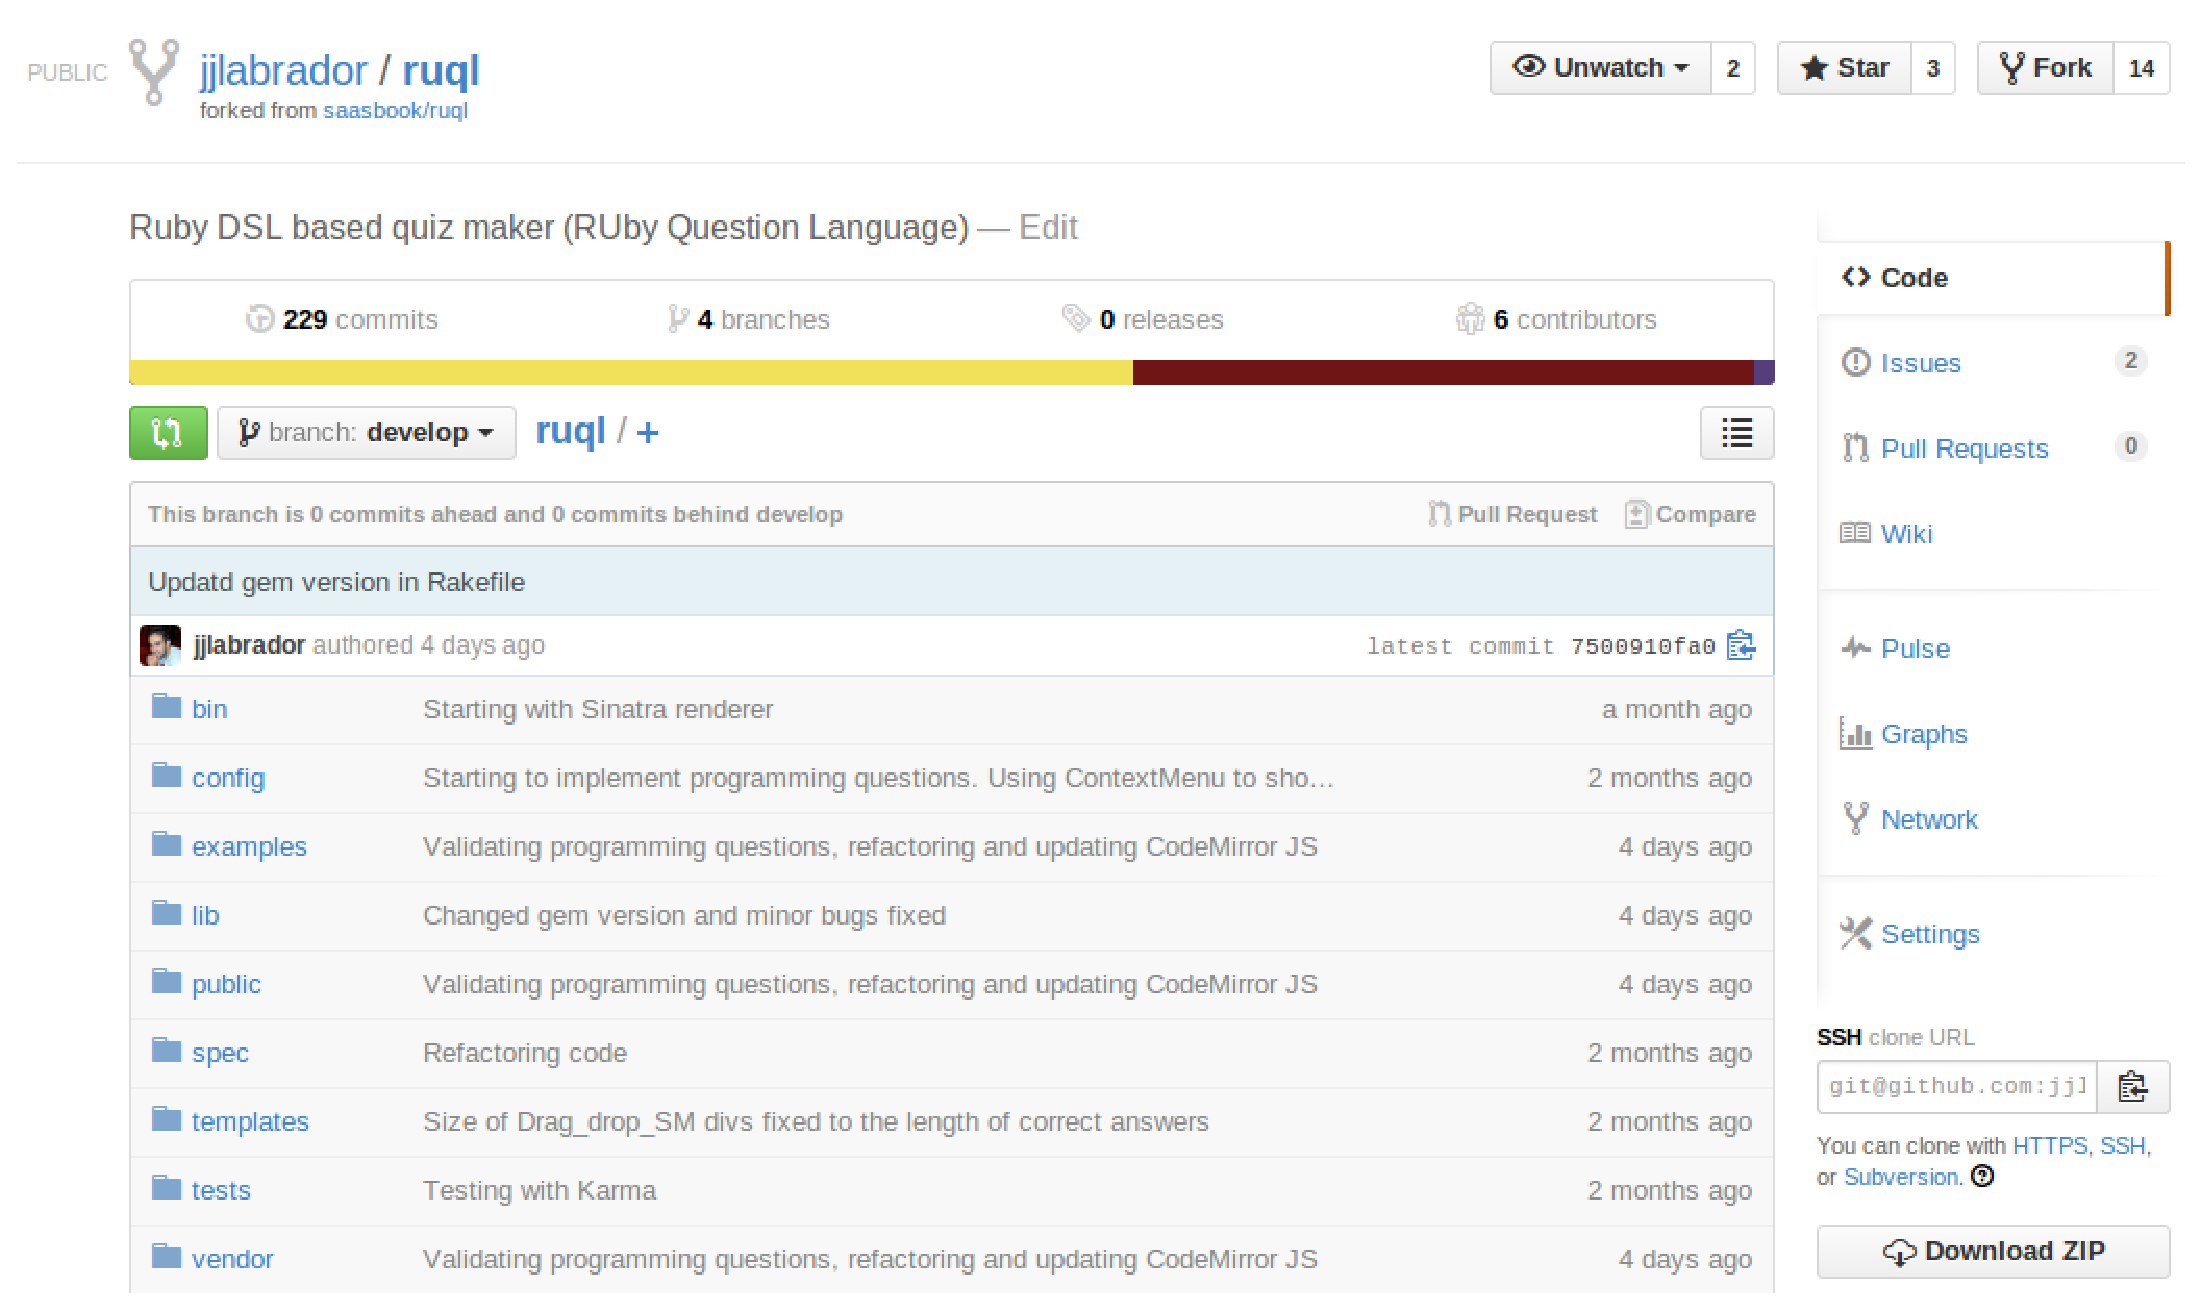
\includegraphics[width=\textwidth,height=0.58\textwidth]{images/github1.eps}
\caption{Captura del repositorio de la gema en GitHub}
\label{fig:github1}
\end{center}
\end{figure}

El trabajo se divid\'{\i}a en ramas, de modo que la versi\'on estable de la aplicaci\'on (\textit{rama master}) quedara aislada de la 
versi\'on en desarrollo (\textit{rama develop}).

\begin{figure}[H]
\begin{center}
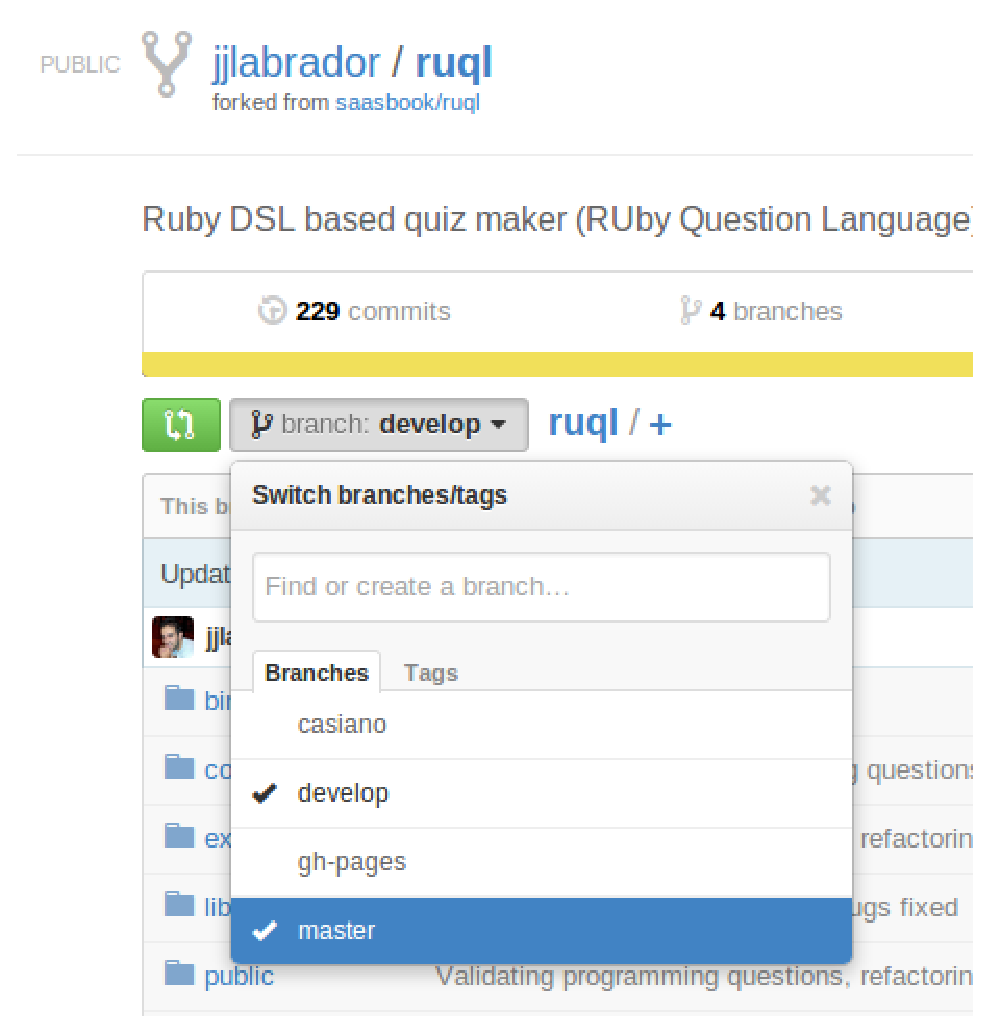
\includegraphics[width=0.47\textwidth]{images/github5.eps}
\caption{Ramas del repositorio propio}
\label{fig:github5}
\end{center}
\end{figure}

GitHub tambi\'en ha servido para mantener contacto con el creador de la \ceit{gema} e indicarle mi intenci\'on de mejorar su gema en mi
Trabajo de Fin de Grado. \'El ha estado al tanto de mi progreso y tras solicitarle \cei{Pull Requests} con mejoras y correcciones
de su gema me ha convertido en colaborador de su \ceit{repositorio}.

\begin{figure}[H]
\begin{center}

\includegraphics[width=1\textwidth]{images/github2.eps}
\caption{Pull Request aceptado y cerrado}
\label{fig:github2}
\end{center}
\end{figure}

\begin{figure}[H]
\begin{center}
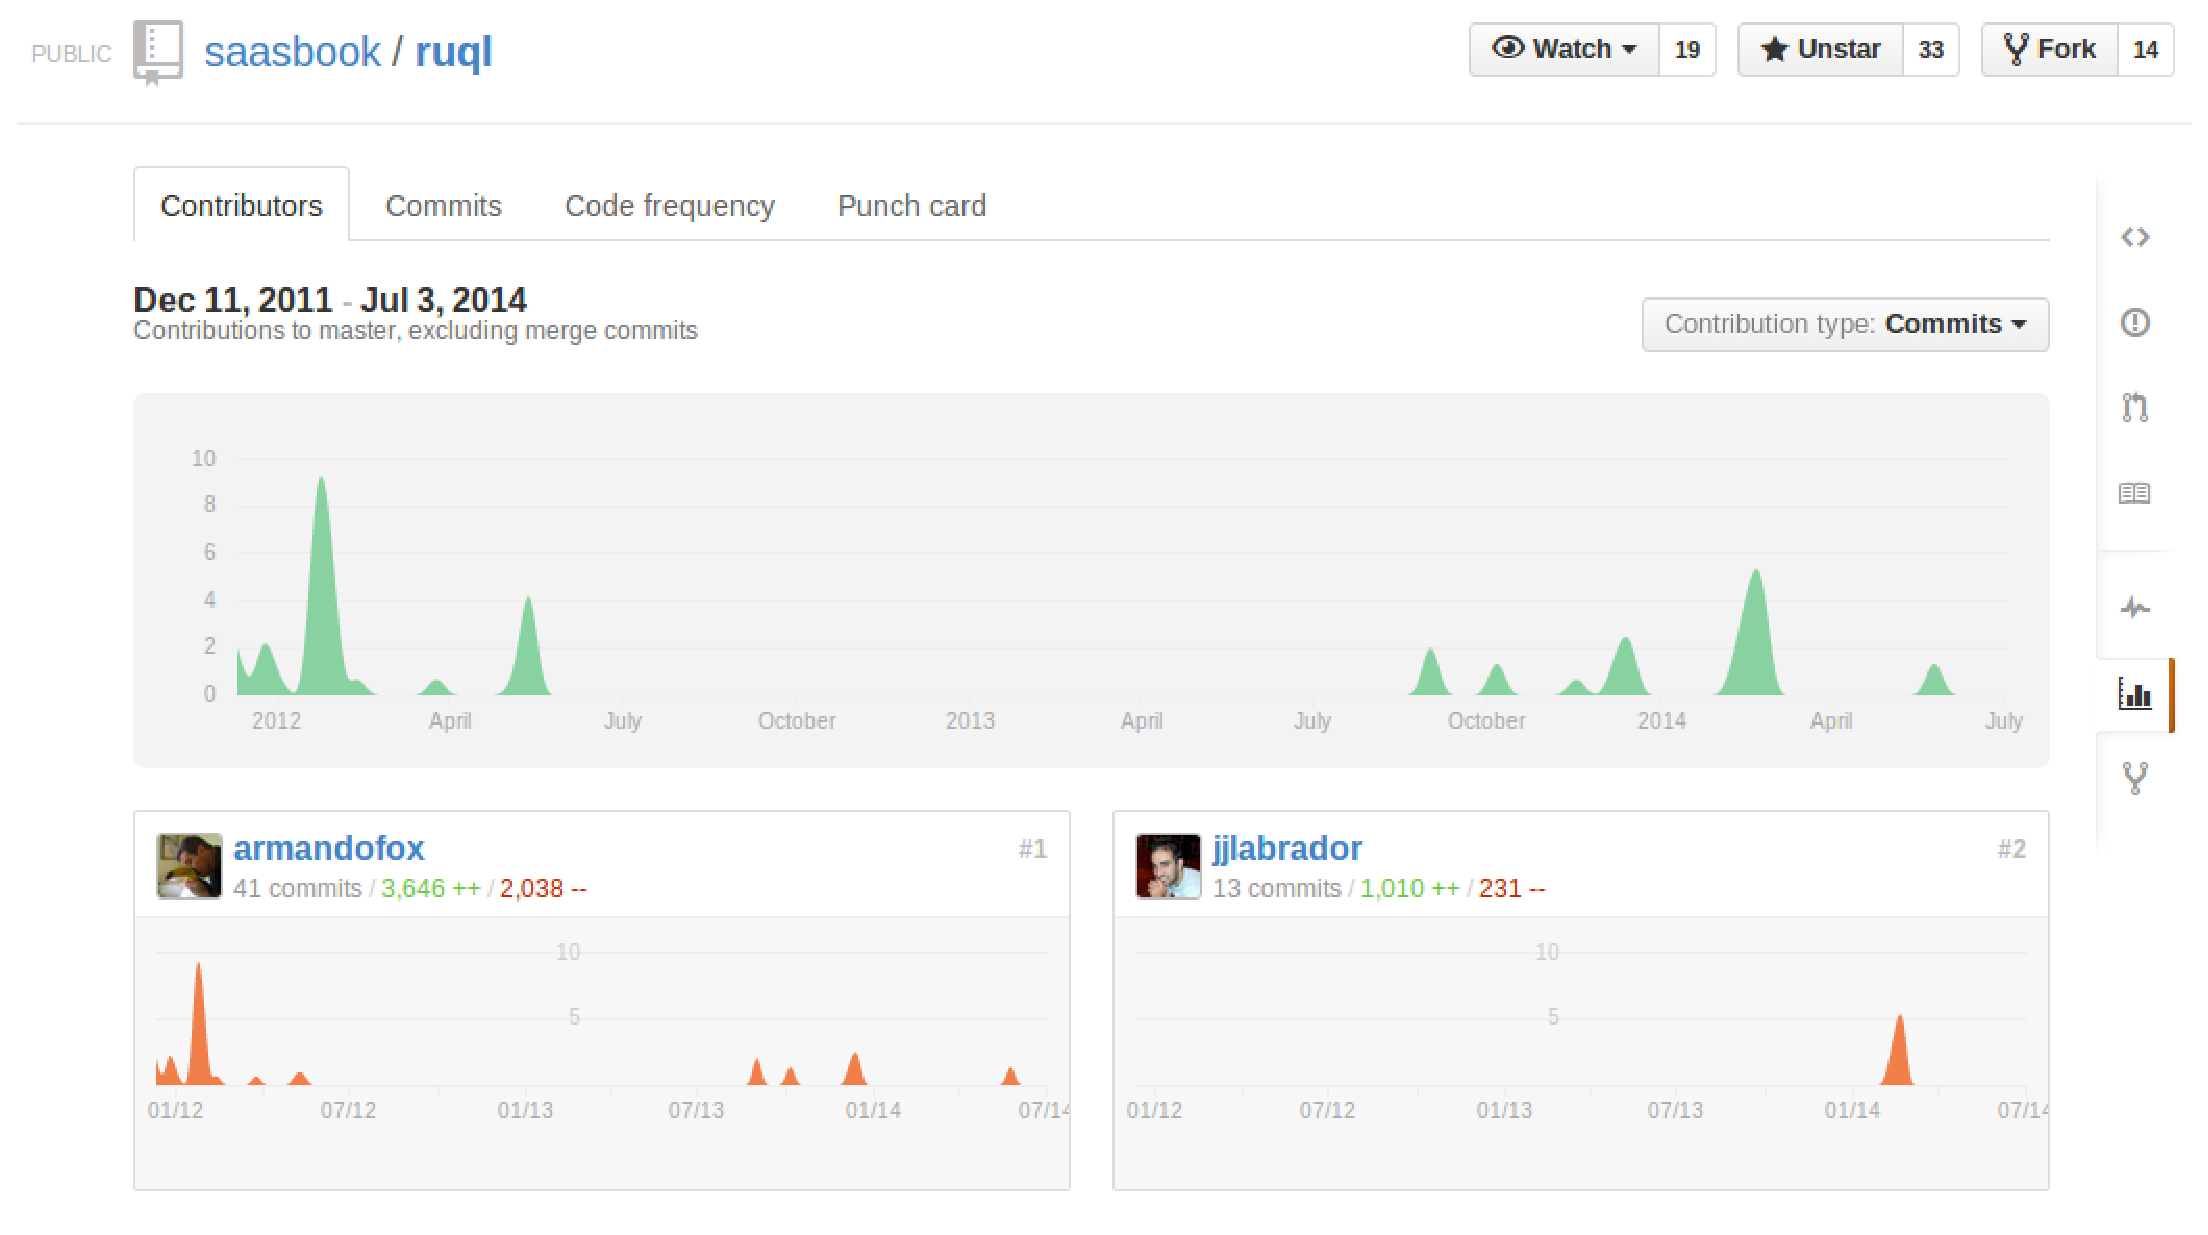
\includegraphics[width=1\textwidth]{images/github3.eps}
\caption{Contribuciones hechas al repositorio original}
\label{fig:github3}
\end{center}
\end{figure}

Las nuevas funcionalidades que han ido surgiendo, as\'{\i} como los problemas detectados, se anotaban en el apartado de \cei{issues}
con el fin de que quedara constancia de ello y se reflejara el estado en el que se encontraba cada uno.
\newpage

\begin{figure}[H]
\begin{center}
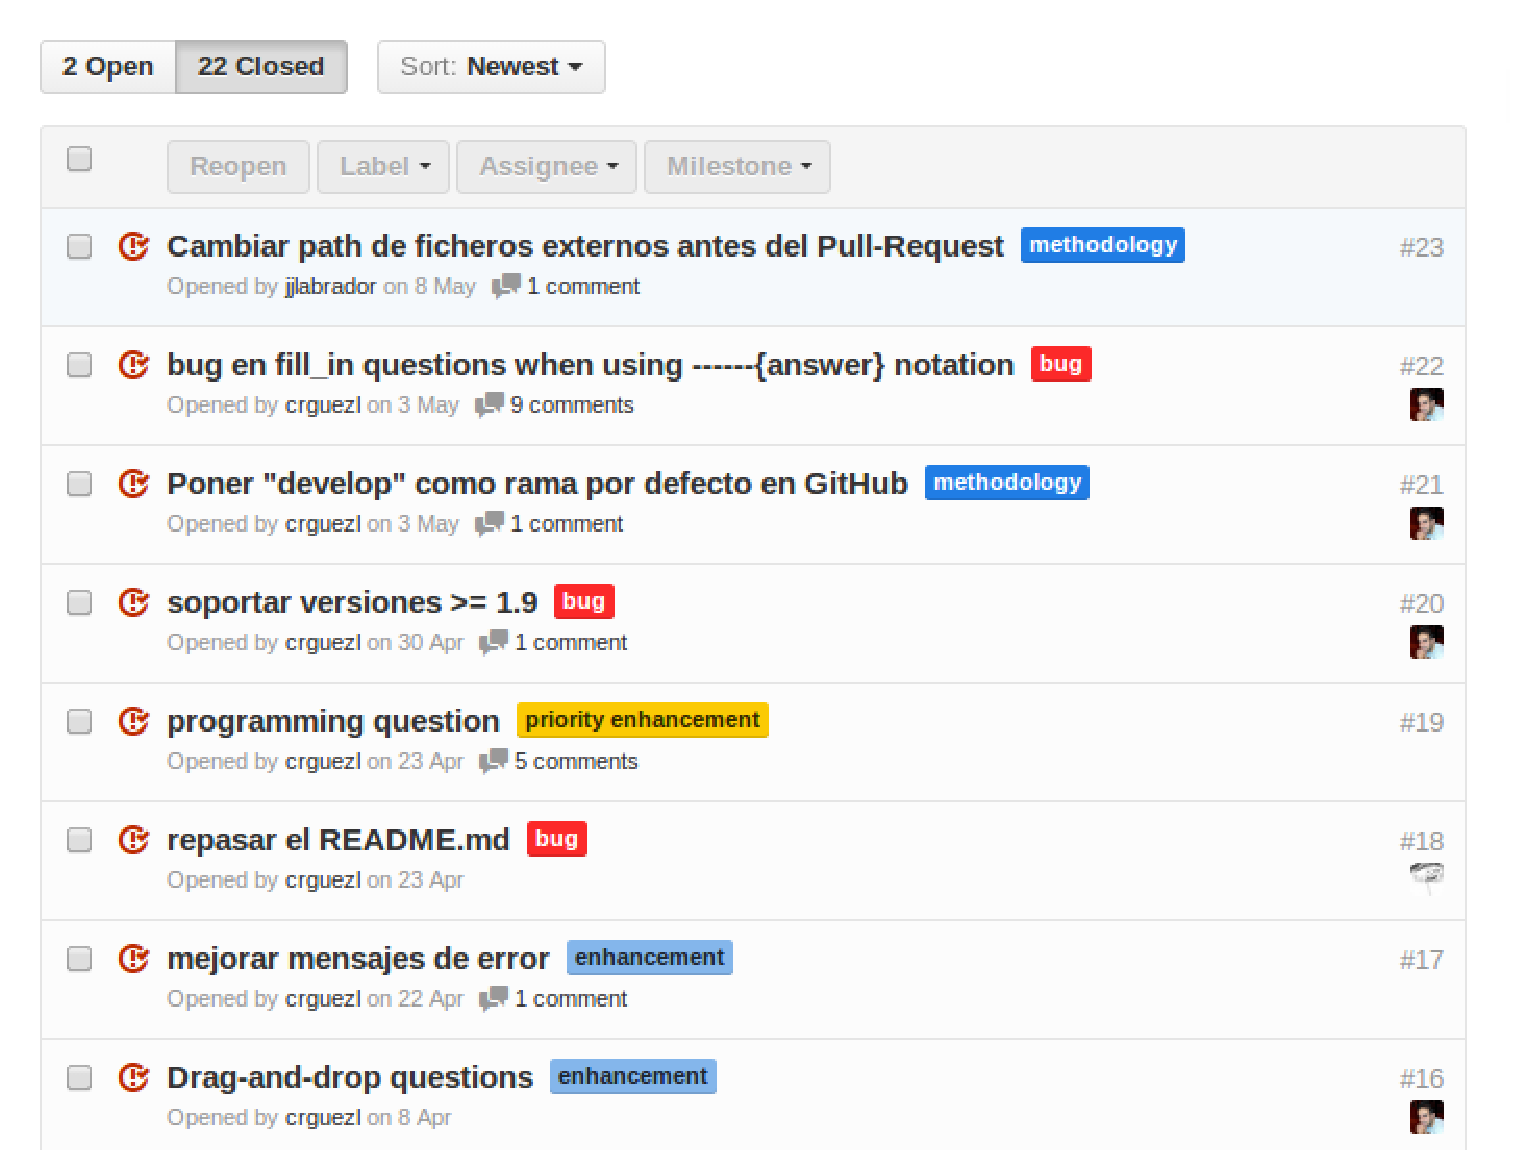
\includegraphics[width=1\textwidth]{images/github4.eps}
\caption{Apartado de issues cerrados}
\label{fig:github4}
\end{center}
\end{figure}

%---------------------------------------------------------------------------------
\subsection{Testing}
\label{subsec:2.1.2}

Dentro de la metodolog\'{\i}a tambi\'en ha habido etapas de \ceit{testing}, haciendo uso de la metodolog\'{\i}a de \ceit{Desarrollo Dirigido por Pruebas} 
{\bfseries TDD} (Test Driven Development). Se ha empleado la herramienta \cei{Spec} para los \ceit{test} en \ceit{Ruby} y se han usado los \ceit{\ref{apend1:framework}}
\cei{Mocha}, \cei{Chai} y \cei{Karma} para los test del \ceit{HTML} y el \ceit{JavaScript}.

%---------------------------------------------------------------------------------
\subsection{Experiencia de usuario}
\label{subsec:2.1.3}

Por otra parte, el tutor del Trabajo de Fin de Grado ha hecho pruebas reales usando los prototipos de la aplicaci\'on con alumnos de sus asignaturas.
De este modo, se comprobaba el funcionamiento de la aplicaci\'on en un entorno real y se recibi\'a un valioso \ceit{feedback} para mejorar en las siguientes
iteraciones.
\bigskip

\section{Resultados}
\label{2:sec:2}

Tras el desarrollo del Trabajo de Fin de Grado, se distinguen tres claros resultados: por un lado tenemos la {\bfseries correci\'on de errores y mejoras
de la gema original}. En segunda instancia, contamos con el \ceit{renderer} \ceis{HtmlForm}, que genera un \ceit{HTML} v\'alido para realizar una autoevaluaci\'on por parte 
del alumnado que adem\'as, le sirve como entrenamiento para afrontar el examen final. Por \'ultimo, contamos con el renderer \ceis{Sinatra}, que genera 
una aplicaci\'on Sinatra correctora de ex\'amenes con todo lo necesario para su \ceit{despliegue} y puesta en funcionamiento.

Se explicar\'an cada uno de estos resultados en los siguientes cap\'{\i}tulos de la memoria.
